\documentclass[conference]{IEEEtran}
\usepackage[T1]{fontenc}
\usepackage[utf8]{inputenc}

\usepackage{fullpage}
\usepackage[french]{babel}
\usepackage{graphicx}

\title{PROJ: DeepVoice}

\author{Rémi Hutin \and Rémy Sun \and Raphael Truffet}

\begin{document}

\maketitle


\begin{figure}[!h]
    \centering
    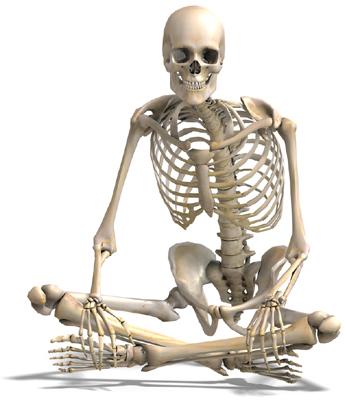
\includegraphics[scale=2]{squelette.jpg}
\end{figure}

\section{Introduction}

\section{Sound signals}

\subsection{Cepstral analysis}

The speech signal of a locutor is hardly suitable for statistical modeling or the calculation of a distance.
In order to obtain a representation which is more compact and less redundant, we use a cepstral representation of the speech.

The cepstrum of a signal $x(t)$ is defined by :

$$C(x(t)) = F^{-1}(\ln(|F(x(t))|)$$

\subsection{GMMs}

\subsection{Supervectors and i-vectors}

\subsection{Previous works}

\section{Use of neuronal networks}

\subsection{Formal neuron}

\paragraph{Neuron?}
A neuron can be thought of as a function which takes an $n$-dimensional vector $A$ as input and returns a scalar $e$ as output. This function typically has two internal parameters which are a bias $b$ and a weight-matrix $W$. The function starts by calculating $WA+b$ before using a non-linear activation function (such as sigmoid or tanh): $e=f(WA+b)$.

\paragraph{Adjusting the function}
Our endgoal is to have the neuron, and by extension the neural network, perform
a certain task. The formal neuron \og learns\fg by adjusting its function to perform better on
this designated task. For simplicity's sake, we will first explain how this
process - called \og backpropagation\fg{} - works with a single neuron.

For instance, suppose we have a bi-dimensional vector given as input and that we
want our neuron to return 1 if its two coordinates are the identical and -1 if
it is not. A natural way to evaluate how accurate our neuron is by looking at the
distance between its output $e$ and the desired result r : d(e)=|e-r|.

We want to modify our neuron/function to minimize this distance. That means
changing $e$, typically by gradient descent on function $d$ derivative. Here,
$\frac{\partial d}{\partial e} = r-e$, which means we want to \og move\fg{} $e$ in this
direction. To this end, we modify our function's two internal parameters $W$ and
$b$. $e$, and by extension $d$, can actually be seen as a function of those two
parameters: $d(W,b)=|e(W,b)-r|$. Therefore $\frac{\partial d}{\partial W}
   = \frac{\partial d}{\partial e}\frac{\partial e}{\partial W}$,
$\frac{\partial d}{\partial b}
   = \frac{\partial d}{\partial e}\frac{\partial e}{\partial b}$. We then only
   need to compute new internal parameters $W'$ and $b'$ with 

\begin{equation}
     W'=W + s\frac{\partial d}{\partial W}=W-s\frac{\partial d}{\partial e}\frac{\partial e}{\partial W}
\end{equation}

\begin{equation}
     b'=b + s\frac{\partial d}{\partial b}=b-s\frac{\partial d}{\partial e}\frac{\partial e}{\partial b}
\end{equation}

What we just demonstrated was a simple backpropagation algorithm called gradient
descent. This method is deeply flawed, but most state of the art backpropagation
methods find their origins in this humble algorithm.

\paragraph{Neuronal network?}

Typically, a neural \textbf{network} is made up of more than a single neuron. A
neural layer refers to multiple neurons working on the same input (or parts of
the same input) and producing an output that can be construed as some form of
concatenation of their respective outputs. This output can be in turn regarded
as an alternate representation of the input. Backpropagation for each neuron
works the same way as it would if it were the only neuron calculating.

The notion of \textbf{deep} learning comes from the fact that the alternate
reprensentation computed by one layer $A$ can be fed as input to another layer $B$.
This allows networks to infer multiple levels of representation, same as one
first processes simple geometrical forms before recognizing more complex
compositions. Backpropagation is straight-forwardly computed on layer $B$. It is
computed on layer $A$ by looking at $\frac{\partial d}{\partial input_B}$
instead of $\frac{\partial d}{\partial e}$
\subsection{Autoencoders}

\paragraph{A default goal}
[We bypass the need for labels by defaulting to an objective that does not require additional information on the input]

\paragraph{Structure}
[Basic canvas of what an autoencoder might look like]

\paragraph{Why use autoencoders?}
[Discussion on generalization processes and denoising autoencoders, explanation of our basic idea and tying it up with the projection issue we are tackling]

\subsection{Tied weight autoencoder}

\paragraph{Architecture}
[Explanation]

\paragraph{Good results}
[Vedran's paper?]

\section{Method}




\end{document}
